%
% parallelogramm.tex
%
% (c) 2018 Prof Dr Andreas Müller, Hochschule Rapperswil
%
\documentclass[tikz]{standalone}
\usepackage{times}
\usepackage{amsmath}
\usepackage{txfonts}
\usepackage[utf8]{inputenc}
\usepackage{graphics}
\usepackage{color}
\usepackage{pifont}
\usetikzlibrary{arrows,intersections,math,calc}
\begin{document}

\def\punkt#1{
        \fill[color=white] #1 circle[radius=0.08];
        \draw #1 circle[radius=0.08];
}

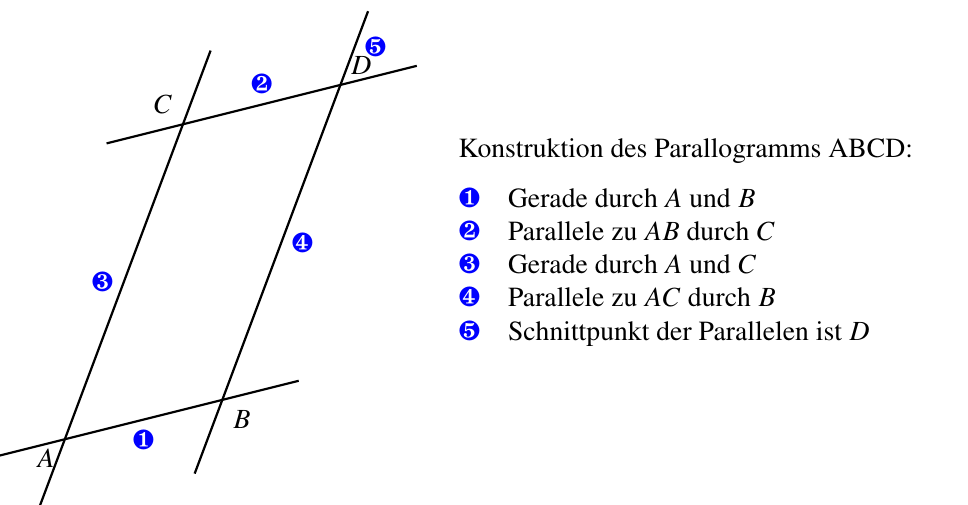
\begin{tikzpicture}[>=latex,thick]

\coordinate (O) at (0,0);
\coordinate (A) at (2,0.5);
\coordinate (B) at (1.5,4);
\coordinate (C) at ($(A)+(B)$);

\draw [shorten >= -1cm, shorten <= -1cm] (O) to (A);
\draw [shorten >= -1cm, shorten <= -1cm] (O) to (B);

\draw [shorten >= -1cm, shorten <= -1cm] (B) to (C);
\draw [shorten >= -1cm, shorten <= -1cm] (A) to (C);

\punkt{(O)} \node at (O) [below left] {$A$};
\punkt{(A)} \node at (A) [below right] {$B$};
\punkt{(B)} \node at (B) [above left] {$C$};
\punkt{(C)} \node at (C) [above right] {$D$};

\node[color=blue] at ($0.5*(A)$) [below] {\ding{182}};
\node[color=blue] at ($(B)+0.5*(A)$) [above] {\ding{183}};
\node[color=blue] at ($0.5*(B)$) [left] {\ding{184}};
\node[color=blue] at ($(A)+0.5*(B)$) [right] {\ding{185}};
\node[color=blue] at ($1.05*(C)$) [above right] {\ding{186}};

\node at (8,2.5) {%
\begin{minipage}{6cm}
\parindent0pt
Konstruktion des Parallogramms ABCD:\\[6pt]
{\color{blue}\ding{182}}\quad Gerade durch $A$ und $B$\\
{\color{blue}\ding{183}}\quad Parallele zu $AB$ durch $C$\\
{\color{blue}\ding{184}}\quad Gerade durch $A$ und $C$\\
{\color{blue}\ding{185}}\quad Parallele zu $AC$ durch $B$\\
{\color{blue}\ding{186}}\quad Schnittpunkt der Parallelen ist $D$
\end{minipage}};

\end{tikzpicture}

\end{document}

